\documentclass[12pt, a4paper, oneside]{ctexart}
\usepackage{amsmath, amsthm, amssymb, bm, graphicx, hyperref, mathrsfs}
\usepackage{makecell}
\usepackage{color}
\usepackage{geometry}%设置整体页面布局
\usepackage{pdfpages}
\geometry{a4paper}
\geometry{left=2cm,right=2cm,top=2.54cm,bottom=2.54cm}%word常规页边距
% \geometry{left=1.27cm,right=1.27cm,top=1.27cm,bottom=1.27cm}%word窄页边距
\setlength{\headheight}{13pt}%避免warning
\title{\textbf{HW2}}
\author{范潇\quad2254298}
\date{\today}
\linespread{1.5}
\newcounter{problemname}
\newenvironment{problem}[1]{\stepcounter{problemname}\par\noindent\textbf{题目\arabic{problemname}. (#1)}}{}
\newenvironment{solution}{\par\noindent\textbf{解答. }}{\\\par}
\newenvironment{note}{\par\noindent\textbf{题目\arabic{problemname}的注记. }}{\\\par}

\begin{document}

\maketitle

\begin{problem}{传教士与野人问题}
    \begin{enumerate}
        \item 对该问题形式化并画出完整的状态空间图。
        \item 应用合适的搜索算法求出该问题的最优解。对于这个问题检查重复状态是个好主意吗?
        \item 这个问题的状态空间很简单,你认为是什么导致人们求解它很困难?
    \end{enumerate}
\end{problem}
\begin{solution}
形式化:
\begin{itemize}
    \item 状态:该问题中的一个状态可以用一个三元组 $(m,c,b)$来表示,其中 $m,c$分别表示起始岸上的传教士个数以及野人个数;$b$为 $1$时,代表船停靠在起始岸,为 $0$则停靠在目标岸。
    \item 初始状态: $(3,3,1)$
    \item 行动:两岸之一上的人乘船到另一岸上,用一个两元组 $(\Delta m,\Delta c)$表示。 $\Delta m,\Delta c\geq 0,1\leq\Delta m+\Delta c\leq 2$
    \item 转移模型: 如果行动前 $d=1$,则行动后状态更新为 $(m-\Delta m,c-\Delta c,0)$;如果行动前 $d=0$,则行动后状态更新为 $(m+\Delta m,c+\Delta c,1)$。
    \item 目标状态: $(0,0,0)$
    \item 路径耗散: 每次行动的耗散为1
\end{itemize}
% \begin{figure}
%     \centering
%     \begin{tabular}{r|l}
%        (3,3,1) &(3,3,0)\\
%     \hline(3,2,1)&(3,2,0)\\
%     \hline(3,1,1)&(3,1,0)\\
%     \hline(3,0,1)&(3,0,0)\\
%     \hline(2,2,1)&(2,2,0)\\
%     \hline(1,1,1)&(1,1,0)\\
%     \hline(0,3,1)&(0,3,0)\\
%     \hline(0,2,1)&(0,2,0)\\
%     \hline(0,1,1)&(0,1,0)\\
%     \hline(0,0,1)&(0,0,0)\\
%     \end{tabular}
%     \caption{状态空间图}
% \end{figure}
\newpage
\begin{figure}
    \centering
    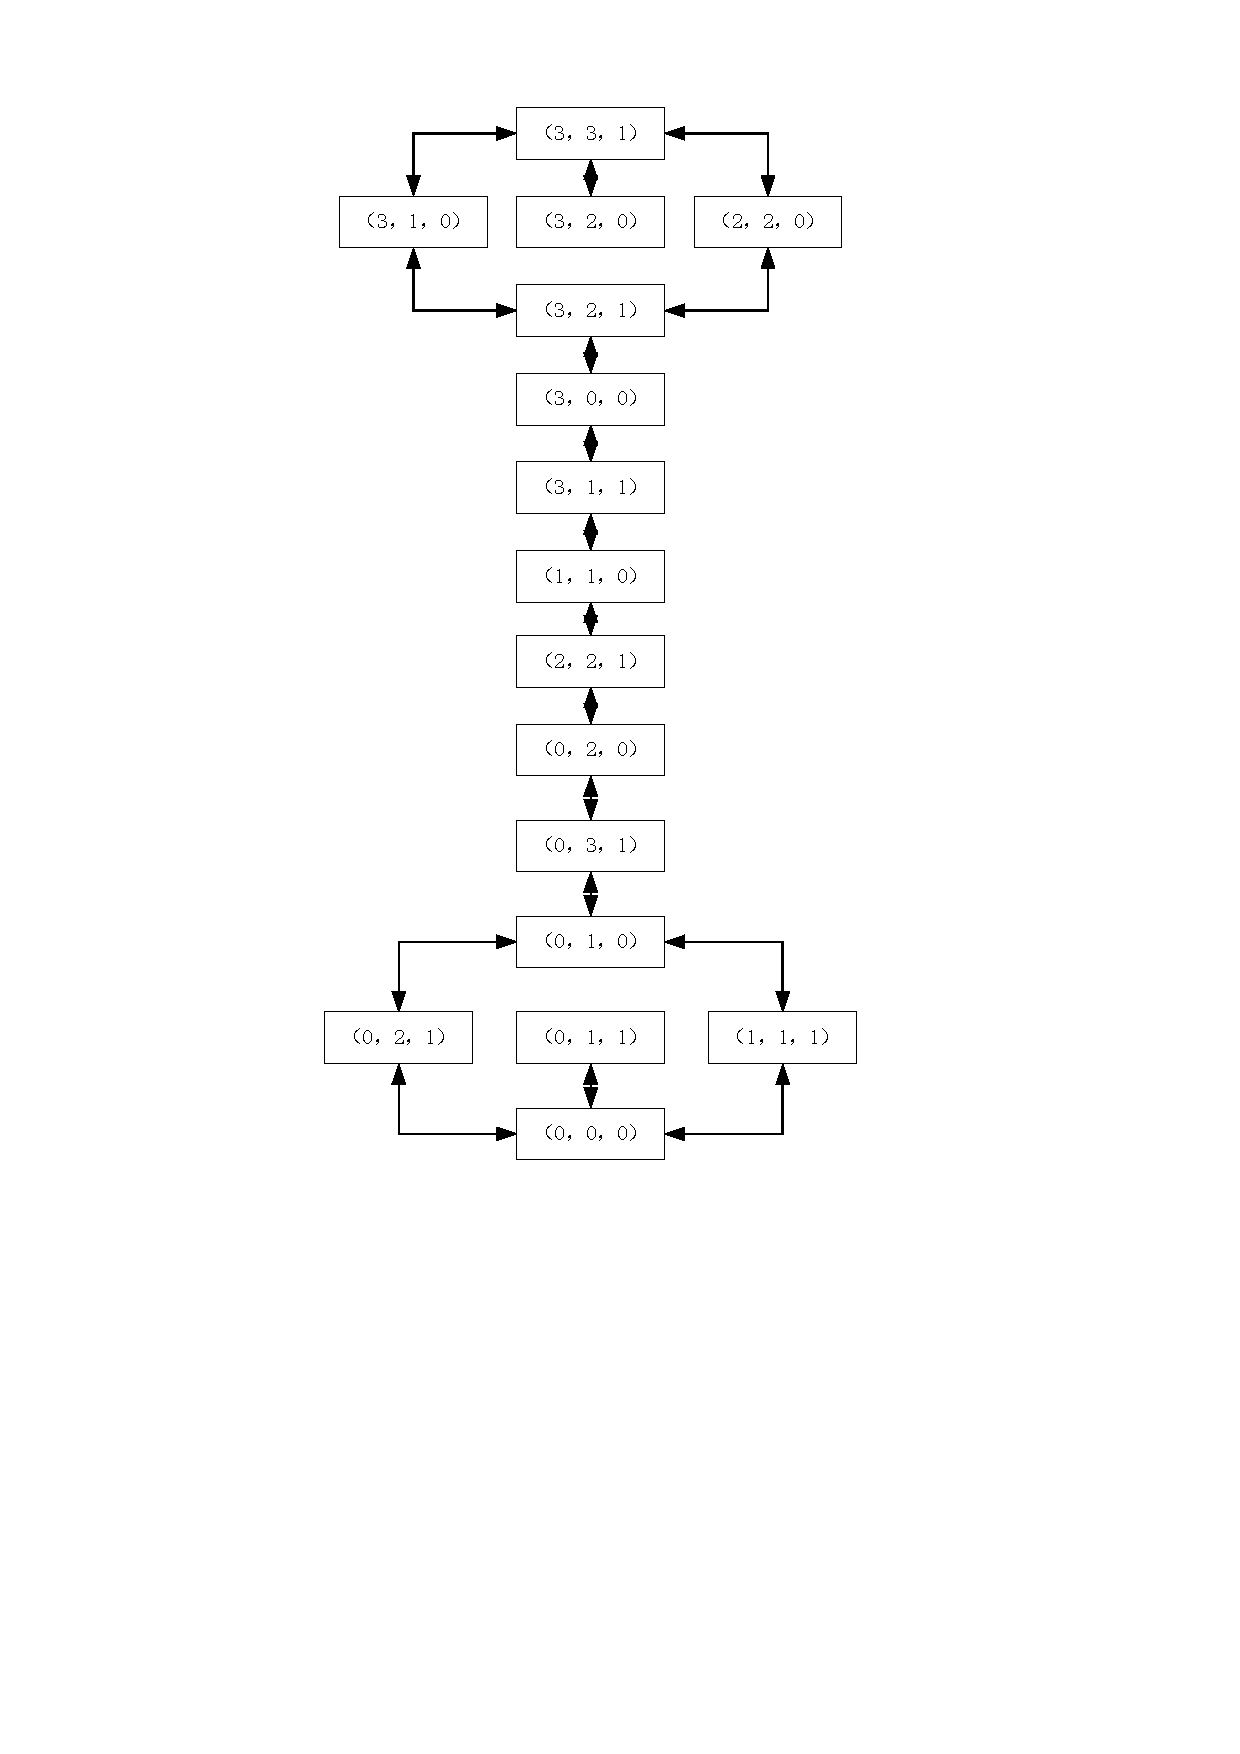
\includegraphics[scale = 0.8]{绘图1.pdf}
\caption{状态空间图}
\end{figure}
该问题的状态空间有限,且每次行动的耗散相同,同时由于对称性,可以从目标状态倒推,所以可以采用双向搜索解决,两个方向的搜索均为广度优先搜索。
因为该问题状态空间较小,且由于具有对称性,极易产生重复状态,所以应当检查重复。

由图2,3可知,一条最短路径为 
\[(3,3,1),(3,1,0),(3,2,1),(3,0,0),(3,1,1),(1,1,0),(2,2,1),(0,2,0),(0,3,1),(0,1,0),(1,1,1),(0,0,0).\]
\begin{figure}
    \centering 
    \begin{tabular}[H]{c|c|c|c|c|c}
        Dir&expand & $frontier_F$ & $frontier_B$ & $reach_F$ & $reach_B$\\
 \hline  F,B &\makecell[c]{(3,3,1)$^0$,\\(0,0,0)$^0$} &\makecell[c]{(3,2,0)$^1$,(3,1,0)$^1$,\\(2,2,0)$^1$}&\makecell[c]{(0,1,1)$^1$,(0,2,1)$^1$,\\(1,1,1)$^1$}&\makecell[c]{(3,3,1)$^0$}&\makecell[c]{(0,0,0)$^0$}\\
 \hline  F &\makecell[c]{(3,2,0)$^1$} &\makecell[c]{(3,1,0)$^1$,(2,2,0)$^1$}&\makecell[c]{(0,1,1)$^1$,(0,2,1)$^1$,\\(1,1,1)$^1$} &\makecell[c]{(3,3,1)$^0$,(3,2,0)$^1$}&\makecell[c]{(0,0,0)$^0$}\\  
 \hline  F &\makecell[c]{(3,1,0)$^1$} &\makecell[c]{(2,2,0)$^1$,(3,2,1)$^2$}&\makecell[c]{(0,1,1)$^1$,(0,2,1)$^1$,\\(1,1,1)$^1$} &\makecell[c]{(3,3,1)$^0$,(3,2,0)$^1$,\\(3,1,0)$^1$}&\makecell[c]{(0,0,0)$^0$}\\
 \hline  F &\makecell[c]{(2,2,0)$^1$} &\makecell[c]{(3,2,1)$^2$}&\makecell[c]{(0,1,1)$^1$,(0,2,1)$^1$,\\(1,1,1)$^1$} &\makecell[c]{(3,3,1)$^0$,(3,2,0)$^1$,\\(3,1,0)$^1$,(2,2,0)$^1$}&\makecell[c]{(0,0,0)$^0$}\\
 \hline  B &\makecell[c]{(0,1,1)$^1$} &\makecell[c]{(3,2,1)$^2$}&\makecell[c]{(0,2,1)$^1$,(1,1,1)$^1$} &\makecell[c]{(3,3,1)$^0$,(3,2,0)$^1$,\\(3,1,0)$^1$,(2,2,0)$^1$}&\makecell[c]{(0,0,0)$^0$,(0,1,1)$^1$}\\
 \hline  B &\makecell[c]{(0,2,1)$^1$} &\makecell[c]{(3,2,1)$^2$}&\makecell[c]{(1,1,1)$^1$,(0,1,0)$^2$} &\makecell[c]{(3,3,1)$^0$,(3,2,0)$^1$,\\(3,1,0)$^1$,(2,2,0)$^1$}&\makecell[c]{(0,0,0)$^0$,(0,1,1)$^1$,\\(0,2,1)$^1$}\\
 \hline  B &\makecell[c]{(1,1,1)$^1$} &\makecell[c]{(3,2,1)$^2$}&\makecell[c]{(0,1,0)$^2$} &\makecell[c]{(3,3,1)$^0$,(3,2,0)$^1$,\\(3,1,0)$^1$,(2,2,0)$^1$}&\makecell[c]{(0,0,0)$^0$,(0,1,1)$^1$,\\(0,2,1)$^1$,(1,1,1)$^1$}\\
 \hline  F &\makecell[c]{(3,2,1)$^2$} &\makecell[c]{(3,0,0)$^3$}&\makecell[c]{(0,1,0)$^2$} &\makecell[c]{(3,3,1)$^0$,(3,2,0)$^1$,\\(3,1,0)$^1$,(2,2,0)$^1$,\\(3,2,1)$^2$}&\makecell[c]{(0,0,0)$^0$,(0,1,1)$^1$,\\(0,2,1)$^1$,(1,1,1)$^1$}\\
 \hline  B &\makecell[c]{(0,1,0)$^2$} &\makecell[c]{(3,0,0)$^3$}&\makecell[c]{(0,3,1)$^3$} &\makecell[c]{(3,3,1)$^0$,(3,2,0)$^1$,\\(3,1,0)$^1$,(2,2,0)$^1$,\\(3,2,1)$^2$}&\makecell[c]{(0,0,0)$^0$,(0,1,1)$^1$,\\(0,2,1)$^1$,(1,1,1)$^1$,\\(0,1,0)$^2$}\\
 \hline  F &\makecell[c]{(3,0,0)$^3$} &\makecell[c]{(3,1,1)$^4$}&\makecell[c]{(0,3,1)$^3$} &\makecell[c]{(3,3,1)$^0$,(3,2,0)$^1$,\\(3,1,0)$^1$,(2,2,0)$^1$,\\(3,2,1)$^2$,(3,0,0)$^3$}&\makecell[c]{(0,0,0)$^0$,(0,1,1)$^1$,\\(0,2,1)$^1$,(1,1,1)$^1$,\\(0,1,0)$^2$}\\
 \hline  B &\makecell[c]{(0,3,1)$^3$} &\makecell[c]{(3,1,1)$^4$}&\makecell[c]{(0,2,0)$^4$} &\makecell[c]{(3,3,1)$^0$,(3,2,0)$^1$,\\(3,1,0)$^1$,(2,2,0)$^1$,\\(3,2,1)$^2$,(3,0,0)$^3$}&\makecell[c]{(0,0,0)$^0$,(0,1,1)$^1$,\\(0,2,1)$^1$,(1,1,1)$^1$,\\(0,1,0)$^2$,(0,3,1)$^3$}\\
    \end{tabular} 
    \caption{双向搜索}
\end{figure}
\begin{figure}
    \centering 
    \begin{tabular}[H]{c|c|c|c|c|c}
        Dir&expand & $frontier_F$ & $frontier_B$ & $reach_F$ & $reach_B$\\
 \hline  F &\makecell[c]{(3,1,1)$^4$} &\makecell[c]{{(1,1,0)$^5$}}&\makecell[c]{(0,2,0)$^4$} &\makecell[c]{(3,3,1)$^0$,(3,2,0)$^1$,\\(3,1,0)$^1$,(2,2,0)$^1$,\\(3,2,1)$^2$,(3,0,0)$^3$,\\(3,1,1)$^4$}&\makecell[c]{(0,0,0)$^0$,(0,1,1)$^1$,\\(0,2,1)$^1$,(1,1,1)$^1$,\\(0,1,0)$^2$,(0,3,1)$^3$}\\
 \hline  B &\makecell[c]{(0,2,0)$^4$} &\makecell[c]{{(1,1,0)$^5$}}&\makecell[c]{(2,2,1)$^5$} &\makecell[c]{(3,3,1)$^0$,(3,2,0)$^1$,\\(3,1,0)$^1$,(2,2,0)$^1$,\\(3,2,1)$^2$,(3,0,0)$^3$,\\(3,1,1)$^4$}&\makecell[c]{(0,0,0)$^0$,(0,1,1)$^1$,\\(0,2,1)$^1$,(1,1,1)$^1$,\\(0,1,0)$^2$,(0,3,1)$^3$,\\(0,2,0)$^4$}\\
 \hline  F &\makecell[c]{{(1,1,0)$^5$}} &\makecell[c]{{\textcolor{red}{(2,2,1)$^6$}}}&\makecell[c]{\textcolor{red}{(2,2,1)$^5$}} &\makecell[c]{(3,3,1)$^0$,(3,2,0)$^1$,\\(3,1,0)$^1$,(2,2,0)$^1$,\\(3,2,1)$^2$,(3,0,0)$^3$,\\(3,1,1)$^4$,(1,1,0)$^5$}&\makecell[c]{(0,0,0)$^0$,(0,1,1)$^1$,\\(0,2,1)$^1$,(1,1,1)$^1$,\\(0,1,0)$^2$,(0,3,1)$^3$,\\(0,2,0)$^4$}\\
% \hline  B &\makecell[c]{(2,2,1)$^5$} &\makecell[c]{{(2,2,1)$^6$}}&\makecell[c]{(1,1,0)$^6$} &\makecell[c]{(3,3,1)$^0$,(3,2,0)$^1$,\\(3,1,0)$^1$,(2,2,0)$^1$,\\(3,2,1)$^2$,(3,0,0)$^3$,\\(3,1,1)$^4$,(1,1,0)$^5$}&\makecell[c]{(0,0,0)$^0$,(0,1,1)$^1$,\\(0,2,1)$^1$,(1,1,1)$^1$,\\(0,1,0)$^2$,(0,3,1)$^3$,\\(0,2,0)$^4$,(2,2,1)$^5$}\\
% \hline  F &\makecell[c]{(2,2,1)$^6$} &\makecell[c]{\textcolor{red}{(0,2,0)$^7$}}&\makecell[c]{(1,1,0)$^6$} &\makecell[c]{(3,3,1)$^0$,(3,2,0)$^1$,\\(3,1,0)$^1$,(2,2,0)$^1$,\\(3,2,1)$^2$,(3,0,0)$^3$,\\(3,1,1)$^4$,(1,1,0)$^5$,\\(2,2,1)$^6$}&\makecell[c]{(0,0,0)$^0$,(0,1,1)$^1$,\\(0,2,1)$^1$,(1,1,1)$^1$,\\(0,1,0)$^2$,(0,3,1)$^3$,\\\textcolor{red}{(0,2,0)$^4$},(2,2,1)$^5$}\\
    \end{tabular}
    \caption{双向搜索}
\end{figure}

因为该问题的状态图的边数较多,且容易产生重复,所以解决起来较为困难。
\end{solution}
\end{document}